% !TEX root = ../thesis.tex

\section{Data and Simulation Samples}
\label{sec:samples}

% The need for simulation samples of signal and background
This search uses the proton-proton collision data collected by the CMS detector during Run 2.
The data are collected and stored for analysis after events generate trigger primitives in the detector subsystems and are selected by the L1 Trigger and HLT as described in chapter~\ref{chap:exp}.
We also list the MC signal samples used in the analysis that are based on the BSM models of subsection~\ref{subsec:benchmark}.
Additionally, we list the MC samples that model SM background contributions to the search.

\subsection{Data Samples}

% Data samples
The data used for this work are based on three different sets over the three Run 2 years of 2016, 2017, and 2018.
For each year of Run 2, documentation is available for the luminosity measurements~\cite{CMS-PAS-LUM-17-001,CMS-PAS-LUM-17-004,CMS-PAS-LUM-18-002}.
The full dataset is divided into three sets per year, with contributions from the Single Muon, Single Electron, and MET\footnote{Here, MET denotes missing transverse energy ($\Et^\mathrm{miss}$).
However, this terminology is now deprecated and is instead replaced by missing transverse momentum (\ptmiss).} datasets.
These sets are referred to as primary datasets, which are defined as a collection of events that have passed at least one of a set of HLT paths~\cite{Franzoni2016}.
Such datasets may be overlapping in terms of which specific events are present, as they are constructed around grouping together events that have similar physics content in the final state of the event.
For example, the Single Muon primary dataset contains events in which the HLT reconstructed a single muon originating from TPs that passed through the L1 trigger, as described in figure~\ref{fig:L1Trigger}.

% Data certification
Data collected by CMS are certified by the Data Quality Management (DQM) group~\cite{CMSData}, which receives information from each subdetector group about the quality of data obtained over each data-taking period.
The DQM then reviews the information from each subdetector group and certifies the data that is of sufficiently high quality, with relevant certification information released as golden data certificates.

\subsection{Simulated Samples}
\label{sec:simSamples}

% Overview of simulation samples
This analysis makes use of nine benchmark signal models to simulate the narrow resonances that are considered in the search.
The models used are \ggF/\VBF\GBulktoWWtolnuqqbarpr, \ggF/\VBF\RadtoWWtolnuqqbarpr, \DY/\VBF\WprtoWZtolnuqqbar, \DY\WprtoWHtolnubbbar, and \DY/\VBF\ZprtoWWtolnuqqbarpr.
Additionally, we also use MC samples to simulate the background sources that this analysis takes into account as part of the search.

\subsubsection{Signal Samples}

% Signal samples
The \DY\WprtoWH, \DY\WprtoWZ, and \ggF\GBulktoWW samples are restricted to the semileptonic final state, while the other six samples also contain different final states that are not used in this analysis.
Each signal has different samples with 50,000 events for each year of Run 2, for a total of three sets of samples per signal.
Furthermore, each signal has separate samples with 50,000 events for the following resonance masses\footnote{The 2016 \VBF\ZprtoWW and 2016 \VBF\WprtoWZ sets are the exception to this, lacking mass values below $1.2\unit{TeV}$.}: 0.8, 1, 1.2, 1.4, 1.6, 1.8, 2.0, 2.5, 3.0, 3.5, 4.0, and $4.5\unit{TeV}$.
The 2016 \VBF\ZprtoWW and 2016 \VBF\WprtoWZ samples do not have mass values below $1.2\unit{TeV}$, and some samples have masses that extend from $4.5\unit{TeV}$ to $8\unit{TeV}$ in increments of $0.5\unit{TeV}$.
Each sample also has a resonance width that is set to 0.1\% of the resonance mass to ensure that the narrow-width approximation is met.
The samples for each benchmark signal were generated at leading-order (LO) in QCD with \texttt{MadGraph5\_aMC@NLO} versions 2.2.2 and 2.4.2~\cite{Alwall_2014}.

% GbulktoWW and RadToWW details
The \ggF/\VBF\GBulktoWW model assumes a curvature of $\tilde{k}=0.5$ to ensure that the natural width of the graviton is negligible with respect to the experimental resolution, and the cross sections for \ggF\GBulktoWW are next-to-leading-order (NLO), while those of the \VBF process are LO.
For the \ggF/\VBF\RadtoWW model, the samples are produced assuming $\Lambda_{R}=3\unit{TeV}$ and $k\pi r_c=35$, with NLO cross sections used for the \ggF process.
The \VBF process does not have any theoretical cross sections available for the bulk scenario, but we use cross sections from a separate RS model.

% ZprtoWW, WprtoWZ, and WprtoWH details
The LO cross sections in the HVT model B are used for \DY\ZprtoWW, \DY\WprtoWZ, and \DY\WprtoWH, with coupling constants given by $g_V=3$, $c_H=-0.98$, and $c_F=1.02$.
In this model, the resonances have large branching fractions to vector boson pairs, with fermionic couplings suppressed.
Meanwhile, the \VBF\ZprtoWW and \DY\WprtoWZ samples use cross sections from the HVT model C, with $g_V\approx1$, $c_H\approx1$, and $c_F=0$.
For model C, the HVT resonances are only produced via \VBF and decay to pairs of SM bosons because the fermionic couplings are zero.

\begin{figure}[htbp]
  \centering
  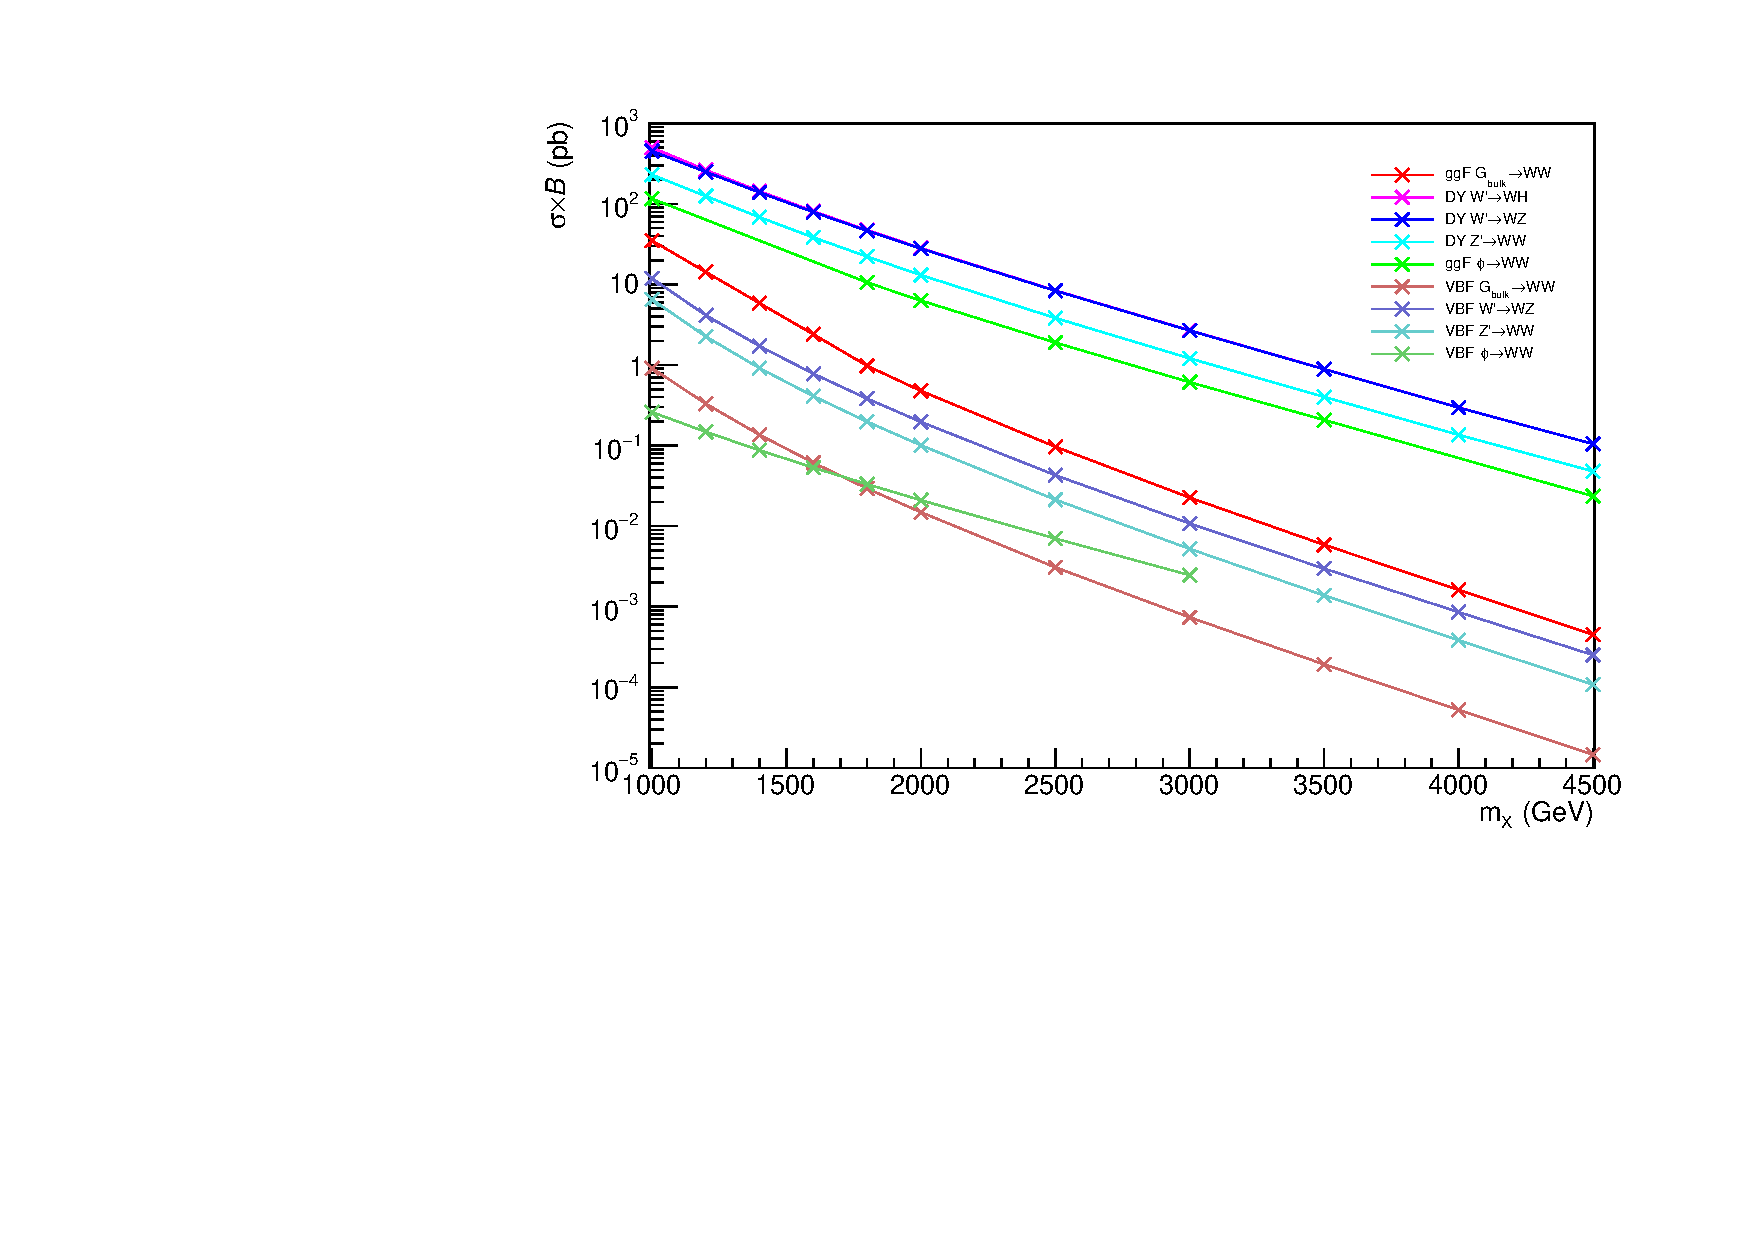
\includegraphics[width=0.75\textwidth]{fig/samples/sigCrossSec.pdf}
  \caption{
    Cross sections multiplied by branching fractions for each of the benchmark signal MC samples as a function of the resonance mass \MX.
  }
  \label{fig:sigCrossSec}
\end{figure}

\subsubsection{Background Samples}

% Background samples
The MC samples used to simulate SM background contributions listed in table~\ref{tab:bkgSamples} along with their cross sections where available.
These include the previously mentioned background processes described in the introduction, consisting of $W$+jets, DY+jets, SM diboson, \bbbar, $t\bar{t}$, single-$t$, and QCD production samples.
The \Wjets process is produced to LO in QCD with \texttt{MadGraph5\_aMC@NLO}.
For the $t\bar{t}$ events, we use samples produced from \texttt{POWHEG} v2~\cite{Nason_2004,Frixione_2007,Alioli_2010,Alioli_2012}, which are rescaled to the NNLO cross section value computed with \texttt{Top++} v2.0~\cite{Czakon_2014}.
The single-$t$ events are generated in the $t$-channel and tW-channel at NLO with \texttt{POWHEG}~\cite{Alioli_2009,Re_2011}.
Finally, the SM diboson processes are produced at NLO with \texttt{MadGraph5\_aMC@NLO} using the merging scheme in reference~\cite{Frederix_2012} for \WZ and \ZZ, and with \texttt{POWHEG} for \WW~\cite{Nason_2014}.

\begin{table}
  \centering
  % !TEX root = ../../thesis.tex
\scriptsize
\begin{tabular}{l|l|l}
  \hline
  Category & Sample name & Total cross section [pb] \\
  \hline
  \hline
  \Wjets & \ttfamily WJetsToLNu\_HT-[MASS]\_[SUFFIX] & \\
  & \ttfamily WJetsToLNu\_HT-[MASS]\_[SUFFIX] & \\
  \hline
  \DY+jets & \ttfamily DYJetsToLL\_M-50\_HT-[MASS]\_[SUFFIX] & \\
  & \ttfamily DYJetsToLL\_M-50\_HT-[MASS]\_[SUFFIX] & \\
  \hline
  \WVt & \ttfamily WWToLNuQQ\_[SUFFIX] & 49.997 \\
  & \ttfamily WWToLNuQQ\_NNPDF31\_[SUFFIX] & 43.53 \\
  & \ttfamily WZTo1L1Nu2Q\_[SUFFIX] & 10.71 \\
  & \ttfamily ZZTo2L2Q\_[SUFFIX] & 3.28 \\
  \hline
  \bbbar & \ttfamily WplusH\_HToBB\_WToLNu\_M125\_[SUFFIX] & 0.1585 \\
  & \ttfamily WminusH\_HToBB\_WToLNu\_M125\_[SUFFIX] & 0.1005 \\
  & \ttfamily ZH\_HToBB\_ZToLL\_M125\_[SUFFIX] & 0.0520 \\
  \hline
  $t\bar{t}$ & \ttfamily TT\_TuneCUETP8M2T4\_[SUFFIX] & 831.76 \\
  & \ttfamily TTTo2L2Nu\_TuneCP5\_PSweights\_[SUFFIX] & 87.31448 \\
  & \ttfamily TTToHadronic\_TuneCP5\_PSweights\_[SUFFIX] & 380.094 \\
  & \ttfamily TTToSemiLeptonic\_TuneCP5\_PSweights\_[SUFFIX] & 364.3508 \\
  \hline
  Single-$t$ & \ttfamily ST\_t-channel\_top\_4f\_inclusiveDecays\_[TuneCP5]\_[SUFFIX] & 136.02 \\
  & \ttfamily ST\_t-channel\_antitop\_4f\_inclusiveDecays\_[TuneCP5]\_[SUFFIX] & 80.95 \\
  & \ttfamily ST\_tW\_antitop\_5f\_inclusiveDecays\_[TuneCP5]\_[SUFFIX] & 35.6 \\
  & \ttfamily ST\_tW\_top\_5f\_inclusiveDecays\_[TuneCP5]\_[SUFFIX] & 35.6 \\
  \hline
  QCD & \ttfamily QCD\_HT[MASS]\_Tune[CUETP8M1/CP5]\_[SUFFIX] & \\
  \hline
\end{tabular}

  \caption{
    Classes of background samples used for Run 2 with total cross sections for each sample used where available.
  }
  \label{tab:bkgSamples}
\end{table}
